\documentclass[leqno]{article}
\usepackage[left=0.5in,right=0.5in]{geometry}
\usepackage[utf8]{inputenc}
\usepackage{amsmath, amsfonts, color, booktabs, centernot, graphicx, fancyhdr}
\setlength\parindent{0pt}
\begin{document}
\title{Kalman Filter Derivation}
\author{Leah Dickstein}

\maketitle

\tableofcontents

\section{Derivation/Proof}

\subsection{Problem Setup:}
\begin{align*}
X[n] &= AX[n-1]+W[n-1]\\
Y[n] &= CX[n]+V[n]\\
\\
\textcolor{red}{X} &\sim N(0, A^{2n} + \sigma_W^2\Sigma_{i=0}^{n-1}A^{2i}\\
\textcolor{red}{Y} &\sim N(0, C^2(A^{2n} + \sigma_W^2\Sigma_{i=0}^{n-1}A^{2i}) + \sigma_V^2\\
\\
X(0) &\sim N(0,1)\\
W[n] &\sim N(0,\Sigma_W)\\
V[n] &\sim N(0,\Sigma_V)
\end{align*}

\subsection{Goal:}
\begin{align*}
\mathbb{E}[X[n+1]|Y^n] &= \hat{X}[n+1]\\
Y^n &= (Y[0] \dots Y[n])\\
\mathbb{E}[X[n+1]|Y^n] &= \sqcup\mathbb{E}[X[n]|Y^{n-1}] + \sqcup(Y[n] - \mathbb{E}[Y[n]|Y^{n-1}]  \\
\end{align*}

\subsection{Equations:}
\begin{align}
L[X|Y] &= \mathbb{E}[X] + \frac{cov(X,Y)}{cov(Y)}(Y-\mathbb{E}[Y])\\
L[X|Y,Z] &= L[X|Y] + L[X|Z-L[Z|Y]]\\
cov(AX,CY) &= Acov(X,Y)C'\\
if V,W \perp cov(V+W) &= cov(V) + cov(W)
\end{align}

\[ \mathbb{E}[X[n+1]|Y^n] = \mathbb{E}[X[n+1]|Y^{n-1}]+\mathbb{E}[X[n+1]|Y[n]-\mathbb{E}[Y[n]|Y^{n-1}] \]

\setcounter{equation}{0}
\subsection{$\mathbb{E}[X[n+1]|Y^{n-1}]$}
\begin{align}
\mathbb{E}[AX[n] + W[n]|Y^{n-1}] &= \mathbb{E}[AX[n]|Y^{n-1}] + \mathbb{E}[W[n]|Y^{n-1}]\\
&= A\hat{X}[n] + \mathbb{E}[W[n]]\\
&= A\hat{X}[n]
\end{align}

\subsection{$\mathbb{E}[Y[n]|Y^{n-1}]$}
\begin{align}
\mathbb{E}[CX[n]+V[n]|Y^{n-1}] &= C\mathbb{E}[X[n]|Y^{n-1}] + \mathbb{E}[V[n]|Y^{n-1}]\\
&= C\hat{X}[n]
\end{align}

\subsection{$\mathbb{E}[X[n+1]|Y[n]-C\hat{X}[n]]$}
\begin{align}
\mathbb{E}[X[n+1]|Y[n]-C\hat{X}[n]] &= \mathbb{E}[AX[n]+W[n]|Y[n]-C\hat{X}[n]]\\
&= \mathbb{E}[AX[n]|Y[n]-C\hat{X}[n]]\\
&= \mathbb{E}[AX[n]-A\hat{X}[n]|Y[n]-C\hat{X}[n]]
\end{align}

\subsection*{Lemma: $Y^{n-1} \perp Y[n]-\mathbb{E}[Y[n]|Y^{n-1}]$}
Strong Induction!\\
\textbf{Base Case:} $cov(Y[0],Y[1]-\mathbb{E}[Y[1]|Y[0]])=0$
\setcounter{equation}{0}
\begin{align}
\mathbb{E}[y[0](cax[0]+cw[0]+v[1]-\frac{ac^2\Sigma_{x[0]}}{\Sigma_{y[0]}}y[0])] &= \mathbb{E}[y[0](cax[0]-\frac{ac^2\Sigma_{x[0]}}{\Sigma_{y[0]}}y[0])]\\
&= \mathbb{E}[(cx[0]+v[0])cax[0]-\frac{ac^2\Sigma_{x[0]}}{\Sigma_{y[0]}}y^2[0]]\\
&= \mathbb{E}[c^2ax^2[0]-\frac{ac^2\Sigma_{x[0]}}{\Sigma_{y[0]}}y^2[0]]\\
&= c^2a\Sigma_{x[0]} - \frac{ac^2\Sigma_{x[0]}}{\Sigma_{y[0]}}\Sigma_{y[0]}\\
&= c^2a\Sigma_{x[0]} - ac^2\Sigma_{x[0]} = 0
\end{align}

\textbf{Inductive Hypothesis:} $cov(Y[n-1],Y[n]-\mathbb{E}[Y[n]|Y[n-1]])=0 \wedge \dots \wedge cov(Y[0],Y[n]-\mathbb{E}[Y[n]|Y[0]])=0$\\

\textbf{Inductive Step:} $cov(Y[n],Y[n+1]-\mathbb{E}[Y[n+1]|Y[n]]) = 0$\\
\[ \mathbb{E}[y[n](cax[n]-\frac{c^2a\Sigma_{x[n]}}{\Sigma_{y[n]}}y[n])] = c^2a\Sigma_{x[n]}-\frac{c^2a\Sigma_{x[n]}}{\Sigma_{y[n]}}\Sigma_{y[n]} = 0 \]

In addition,
\begin{align}
\forall t \leq n,\quad &cov(y[t],y[n+1]-\mathbb{E}[y[n+1]|y[t]]) = 0\\
&= \mathbb{E}[y[t](ca^{n+1-t}x[t]-\frac{c^2a^{n+1-t}\Sigma_{x[t]}}{\Sigma_{y[t]}}y[t])]\\
&= \mathbb{E}[c^2a^{n+1-t}x^2[t]-\frac{c^2a^{n+1-t}\Sigma_{x[t]}}{\Sigma_{y[t]}}y^2[t]]
&= c^2a^{n+1-t}\Sigma_{x[t]}-\frac{c^2a^{n+1-t}\Sigma_{x[t]}}{\Sigma_{y[t]}}\Sigma_{y[t]} = 0
\end{align}

If $t=n+1$,$cov(y[n+1], y[n+1]-\mathbb{E}[y[n+1]|y[n+1]]) = cov(y[n+1], y[n+1]-y[n+1]) = cov(y[n+1], 0) = 0$.\\
The answer is trivial.

\hrulefill

\[ cov(Y^{n-1}, Y[n]-\mathbb{E}[Y[n]|Y^{n-1}]) = \mathbb{E}\left[ [Y[0] \dots Y[n-1] ] \left[Y[n] - \frac{cov(Y[n],Y^{n-1})}{cov(Y^{n-1})} \left[\begin{smallmatrix}Y[0]\\ \vdots \\ Y[n-1] \end{smallmatrix}\right]\right]\right] \]

We have proved for $\forall t < n$ this $=0$, therefore the answer is the 0 vector and we prove the Lemma. Since $\hat{X}[n]=\mathbb{E}[X[n]|Y^{n-1}]$, it is the projection of X onto $Y^{n-1}$. If $Y^{n-1} \perp \tilde{Y}, \hat{X}[n] \perp \tilde{Y}$. We can add if inside the cov() since it's equivalent to adding 0.\\

\[ cov(AX[n] - A\hat{X}[n], CX[n] - C\hat{X}[n]) = Acov(X[n] - \hat{X}[n])C' \]
\[ S_n = cov(X[n] - \hat{X}[n]) \]

\[ cov(Y[n] - C\hat{X}[n]) = cov(CX[n] + V[n] - C\hat{X}[n]) = cov(C(X[n] - \hat{X}[n])) + cov(V[n]) = CS_nC' + \sigma_v^2\]
\[K_n = \frac{AS_nC'}{CS_nC' + \sigma_v^2} \]

\[ \boxed{ \hat{X}[n+1] = \mathbb{E}[X[n+1]|Y^n] = A\hat{X}[n] + \frac{Acov(X[n]-\hat{X}[n])C'}{Ccov(X[n]-\hat{X}[n])C'+\sigma_v^2}\left(Y[n]-C\hat{X}[n]\right) } \]

\section{Simulation}

\subsection{Code}
\begin{verbatim}
%% Kalman Filter (Prediction of Present)
clc
clear all

a = 1; %Test 2,0.5,10
c = 1;
varv = 0.09; %channel noise
varw = 0.04;
n = 50;

%initialize
x = normrnd(0,1,[1,1]); %x[0]
y = c*x+normrnd(0,varv);
xhat = y*c*1/(c^2+varv);
xhatmem = y*c/(c^2+varv);
varx = 1;
vary = c^2+varv;

sigman = varx -2*c*varx^2/vary + c^2*varx^2/vary^2*(c^2*varx+varv);

%sn = a^2+varw - 2*a^2*c^2/(c^2+varv) + a^2*c^4/(c^2+varv)^2 + a^2*c^2/(c^2+varv)^2*varv;


%time passing
for t=1:(n-1)
    w = normrnd(0,varw);
    x = [x a*x(1,t)+w];
    v = normrnd(0,varv);
    y = [y c*x(1,(t+1))+v];
    
    sn = a^2*sigman+varw; %generating sn for this iteration
    kn = sn*c/(c^2*sn+varv);
    xhatmem = [xhatmem a*xhatmem(1,t)+kn*(y(1,t+1)-c*a*xhatmem(1,t))];
    sigman = (1-kn*c)*sn; %generate new sigma_n for next iteration
    %sn = a^2*sigman+varw;
    
    varx = a^2*varx + varw;
    vary = c^2*varx + varv;
    xhat = [xhat y(1,t+1)*c*varx/vary];
end

%hold all
subplot(1,2,1), stem(0:t,x,'k','filled')
%subplot(1,2,1), hold on, stem(0:t,y,'b','filled')
subplot(1,2,1), hold on, stem(0:t,xhat,'r')
subplot(1,2,1), hold on, stem(0:t, xhatmem, 'g','filled')
xlabel('n=time')
legend1 = legend('x','y','xhat','Location','Best');

%subplot(1,2,2), plot(0:t,abs(y/c-x),'g')
subplot(1,2,2), hold on, plot(0:t,abs(xhat-x),'r')
subplot(1,2,2), hold on, plot(0:t,abs(xhatmem-x),'b')
xlabel('n=time')
legend2 = legend('xhat-x','xhatmem-x');
subplot(1,2,2), title('Error')

suptitle(['a= ' num2str(a) '; c= ' num2str(c) '; varv= ' num2str(varv) '; varw= ' num2str(varw)])
\end{verbatim}

\subsection{Plots}
\subsubsection{Example from the Book}
\begin{center}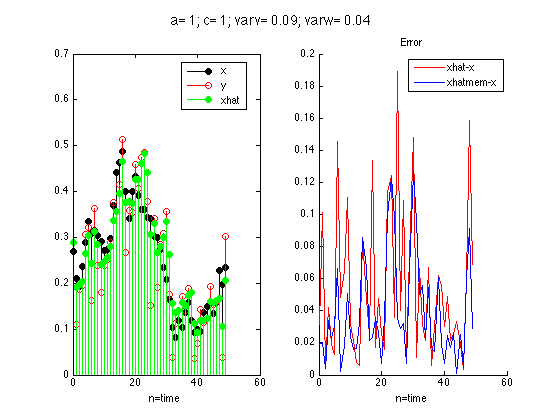
\includegraphics[scale=0.7]{fig1.png}\end{center}

I know this is correct because my $\Sigma_n$ = 0.0432, which perfectly matches the result in the textbook.\\

\begin{center}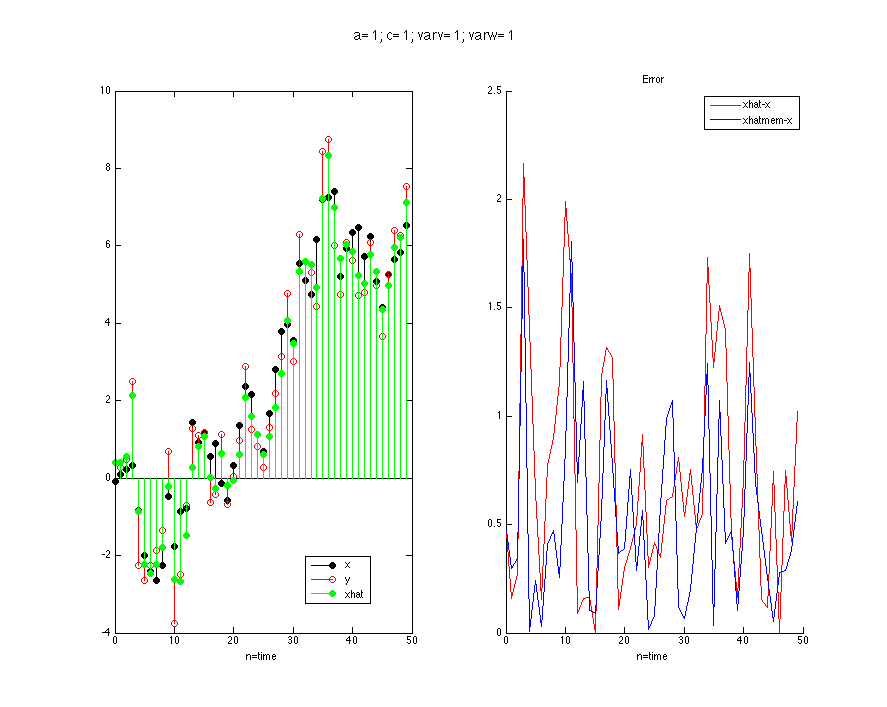
\includegraphics[scale=0.4]{fig2.png}\end{center}
Average Xhat-X = 0.7338; \quad Average Xhatmem - X = 0.5278

\subsubsection{Varying A}
\begin{center}
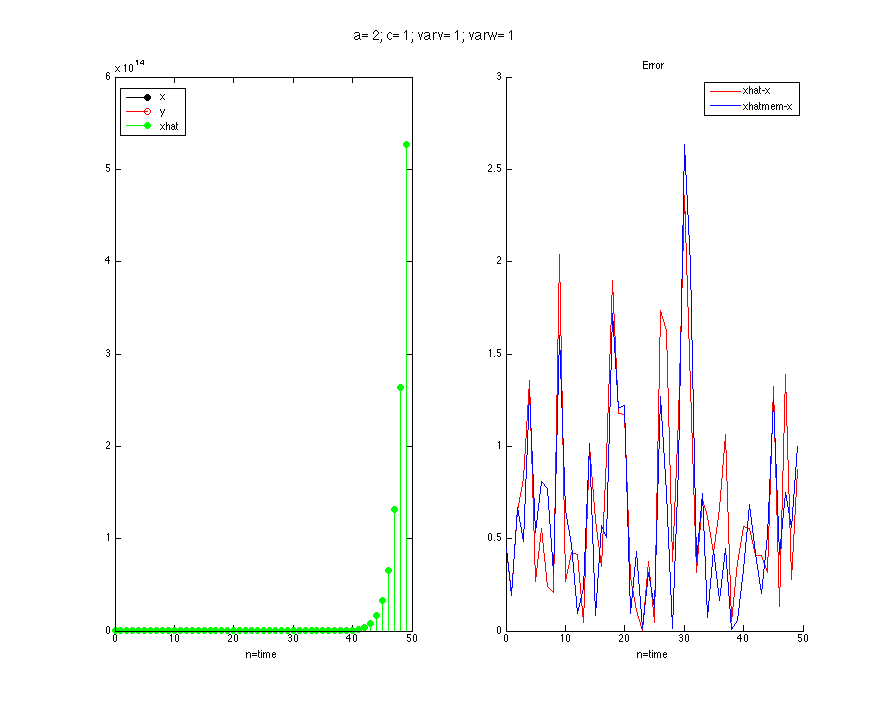
\includegraphics[scale=0.3]{fig3}
\end{center}
Average Xhat - X = 0.6997; \quad Average Xhatmem - X = 0.6376\\

\begin{center}
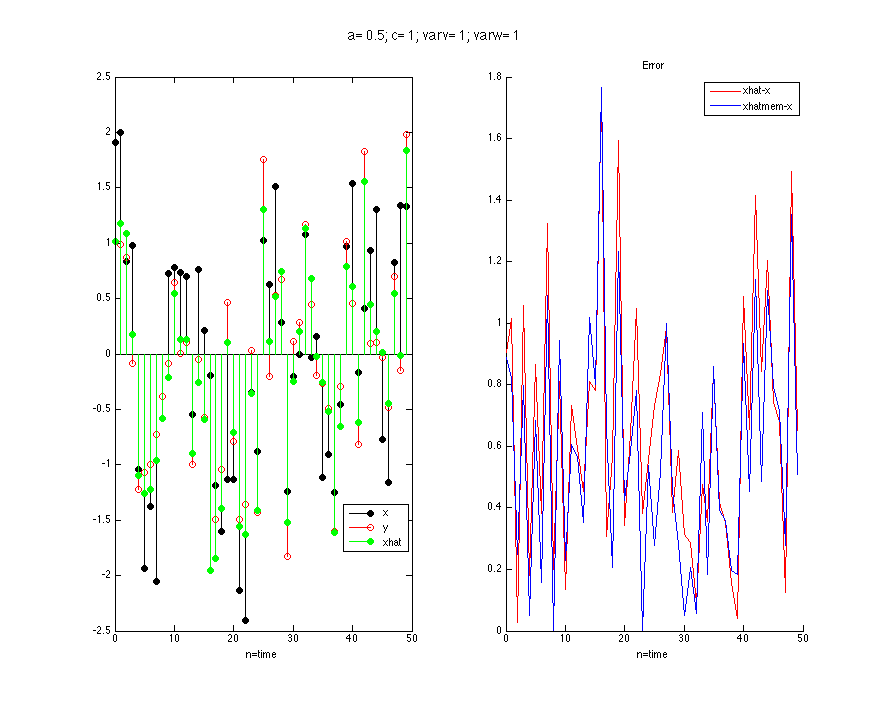
\includegraphics[scale=0.3]{fig4}
\end{center}
Average Xhat - X = 0.6645; \quad Average Xhatmem - X = 0.5791\\

\begin{center}
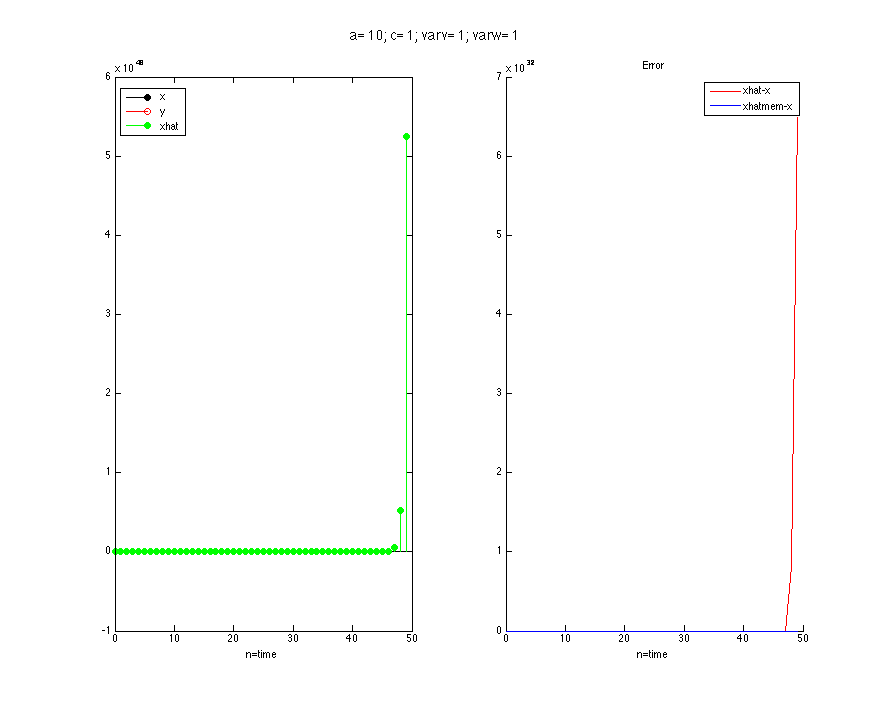
\includegraphics[scale=0.3]{fig5}
\end{center}
Average Xhat - X = $1.4603*10^31$; \quad Average Xhatmem - X = 0.2476 \\

These results indicate that when scaling A larger, Xhat works less efficiently. However, the Kalman Filter (Xhat with Memory) continues to work at around the same level of accuracy.

\subsubsection{Varying C}
\begin{center}
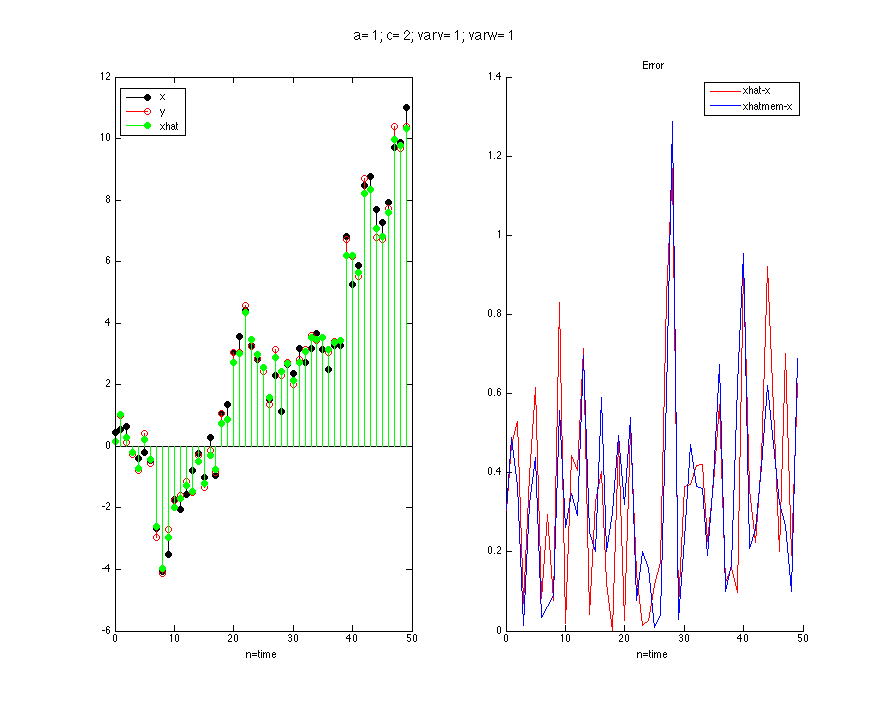
\includegraphics[scale=0.3]{fig6}
\end{center}
Average Xhat - X = 0.3592; \quad Average Xhatmem - X = 0.3486\\

\begin{center}
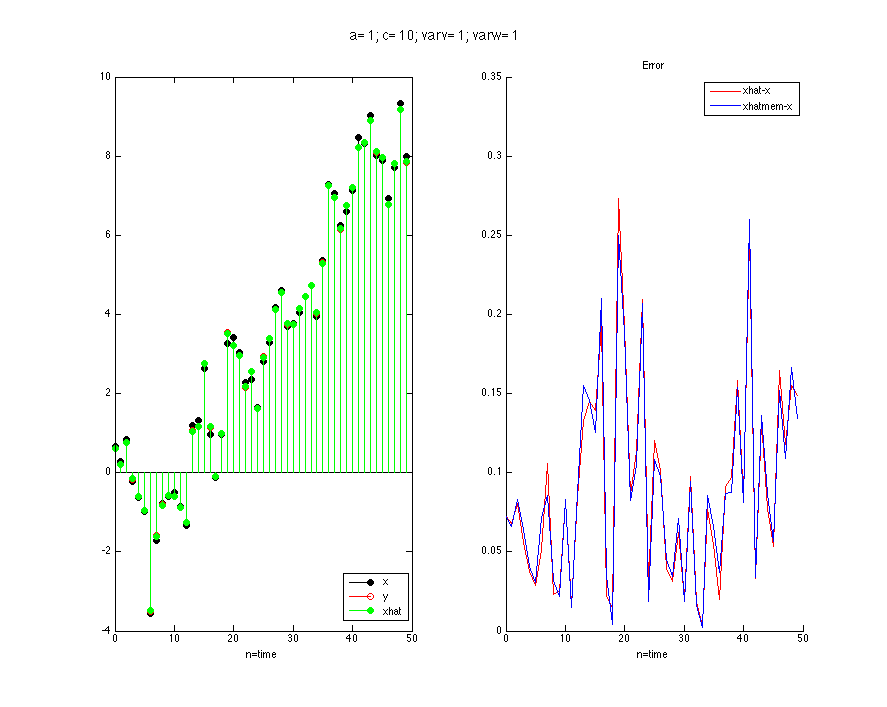
\includegraphics[scale=0.3]{fig7}
\end{center}
Average Xhat - X = 0.0899; \quad Average Xhatmem - X = 0.0900\\

These results indicate changing C decreases error for both Xhat and Xhatmem. In addition, Xhat works just as well if not better as Xhatmem, indicating increasing the power of the signal decreases the benefit of memory.

\subsubsection{Varying Noise}
Increasing Channel Noise:
\begin{center}
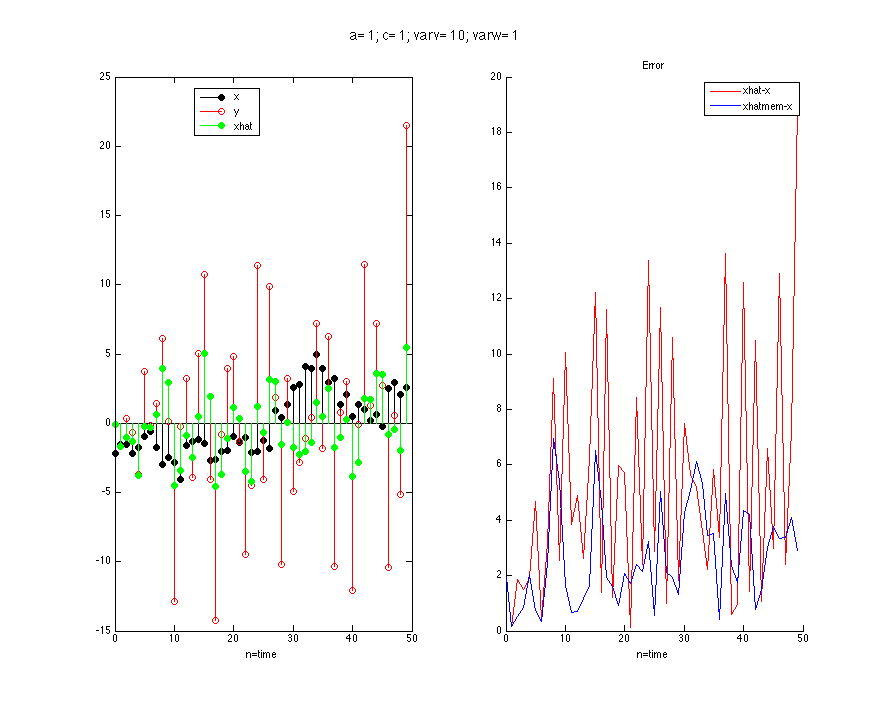
\includegraphics[scale=0.3]{fig8}
\end{center}
Average Xhat - X = 5.4140; \quad Average Xhatmem - X = 2.6805\\

Increasing System Noise:
\begin{center}
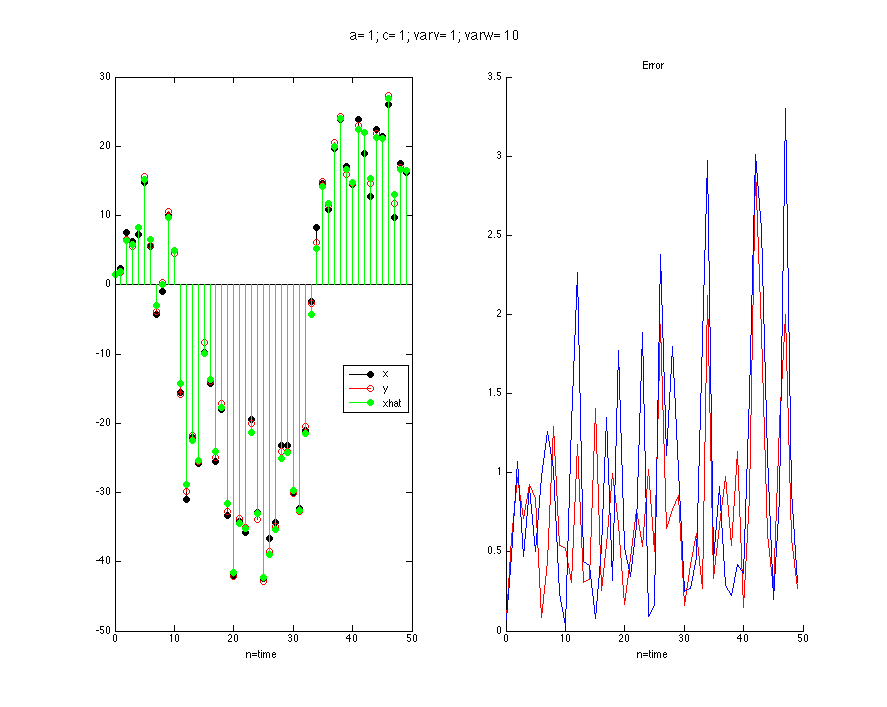
\includegraphics[scale=0.3]{fig9}
\end{center}
Average Xhat - X = 0.7729; \quad Average Xhatmem - X = 0.9512\\

Increasing Channel Noise increases the accuracy gap between Xhat and Xhatmem, with Xhatmem doing better. Increasing System Noise has a larger effect on Xhatmem (the Kalman Filter) than just Xhat, with Xhatmem doing worse. \\

For better results, repeat the experiment $m=100, 10,000$ and calculate/compare average error over $m$ trials.

\section{Predicting the Future}
See KF5\_140614 for the code.

\section{Dynamics}
\subsection{Without Memory}
\subsubsection{Problem Setup:}
\begin{align*}
X_1[n] &\sim N(0, 2^{2n})\\
X_2[n] &\sim N(0, 3^{2n})\\
Y[n] &\sim N(0, 2^{2n} + 3{2n})\\
\end{align*}

Similar to just X[n], $\mathbb{E}[X_1[n]|Y[n]] = \frac{cov(X_1[n])}{cov(Y[n])}Y[n]$.

\subsubsection{Simulation}
\textbf{Code:}
\begin{verbatim}
clc;
clear all;
set(0,'DefaultAxesFontSize', 14);

a1 = 2; %Test 2,0.5,10
a2 = 3;
c1 = 1;
c2 = 1;
n = 10;

%initialize
x1 = normrnd(0,1,[1,1]); %x[0]
x2 = normrnd(0,1,[1,1]);
y = c1*x1+c2*x2;

varx1 = 1;
varx2 = 1;
vary = c1^2+c2^2;

xhat1 = y*c1*varx1/vary;
xhat2 = y*c2*varx2/vary;
sigman1 = (1-c1*varx1/vary)^2*varx1+(c2*varx1/vary)^2*varx2;

%time passing
for t=1:(n-1)
    x1 = [x1 a1*x1(1,t)];
    x2 = [x2 a2*x2(1,t)];
    y = [y c1*x1(1,t+1)+c2*x2(1,t+1)];
    varx1 = a1^2*varx1;
    varx2 = a2^2*varx2;
    vary = c1^2*varx1 + c2^2*varx2;
    xhat1 = [xhat1 y(1,t+1)*c1*varx1/vary];
    xhat2 = [xhat2 y(1,t+1)*c2*varx2/vary];
    sigman1 = [sigman1 (1-c1*varx1/vary)^2*varx1+(c2*varx1/vary)^2*varx2];
end

%hold all
subplot(1,2,1), stem(0:t,x1,'k','filled')
%subplot(1,2,1), hold on, stem(0:t,y,'b','filled')
subplot(1,2,1), hold on, stem(0:t,xhat1,'r','filled')
subplot(1,2,1), hold on, stem(0:t, x2, 'k')
subplot(1,2,1), hold on, stem(0:t, xhat2, 'r')
xlabel('n=time')
legend1 = legend('x1','xhat1','x2','xhat2','Location','Best');

%subplot(1,2,2), stem(0:t,abs(y*c1/(c1+c2)-x1),'b','filled')
subplot(1,2,2), hold on, stem(0:t,xhat1-x1,'r','filled')
%subplot(1,2,2), hold on, stem(0:t, sqrt(sigman1), 'k')
subplot(1,2,2), hold on, stem(0:t,xhat2-x2,'g')
%subplot(1,2,2), hold on, stem(0:t, abs(xhat1-x1+xhat2-x2), 'k', 'filled')
xlabel('n=time')
legend2 = legend('xhat1-x1','xhat2-x2');
subplot(1,2,2), title('Error')

suptitle(['a1= ' num2str(a1) '; a2 = ' num2str(a2)])
\end{verbatim}

\begin{center}
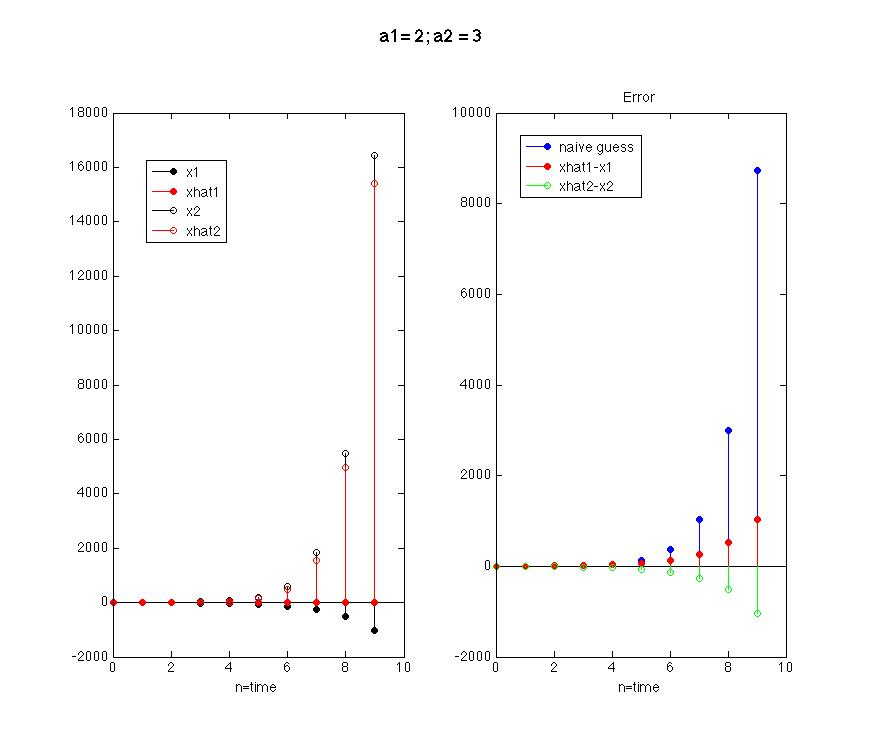
\includegraphics[scale=0.3]{fig1_d}\\
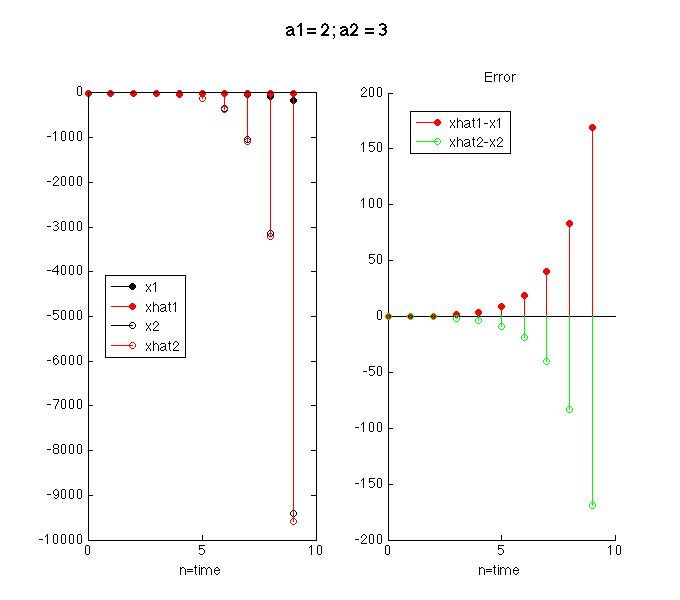
\includegraphics[scale=0.4]{fig2_d}
\end{center}

Here, the error appears to be a concave up, increasing curve. However, if I change the parameters to a1=1, a2 $> 1$, the curve changes shape.

\begin{center}
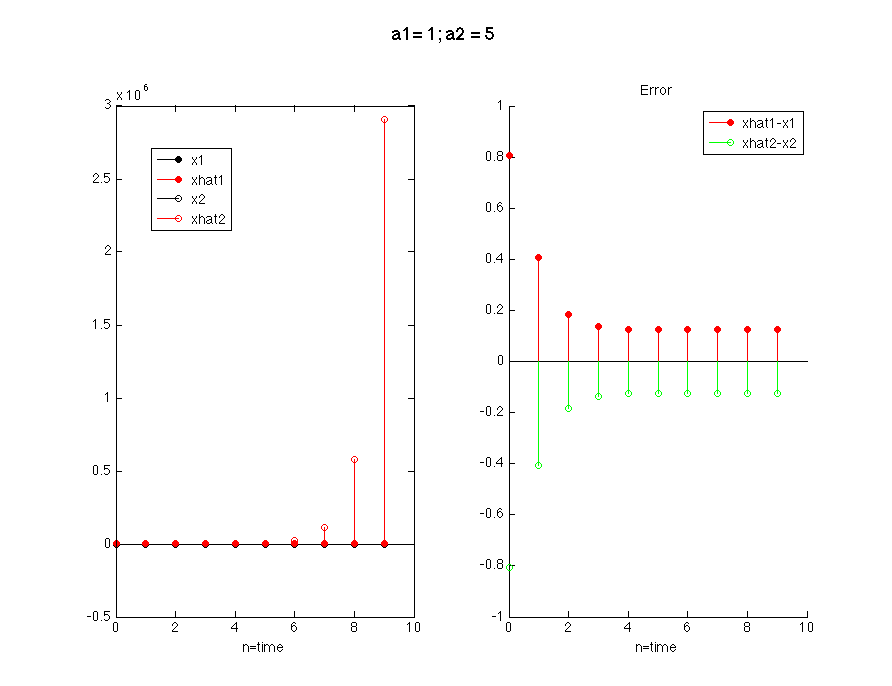
\includegraphics[scale=0.4]{fig3_d}
\end{center}

\end{document}